\begin{figure}[H]
    \begin{center}
        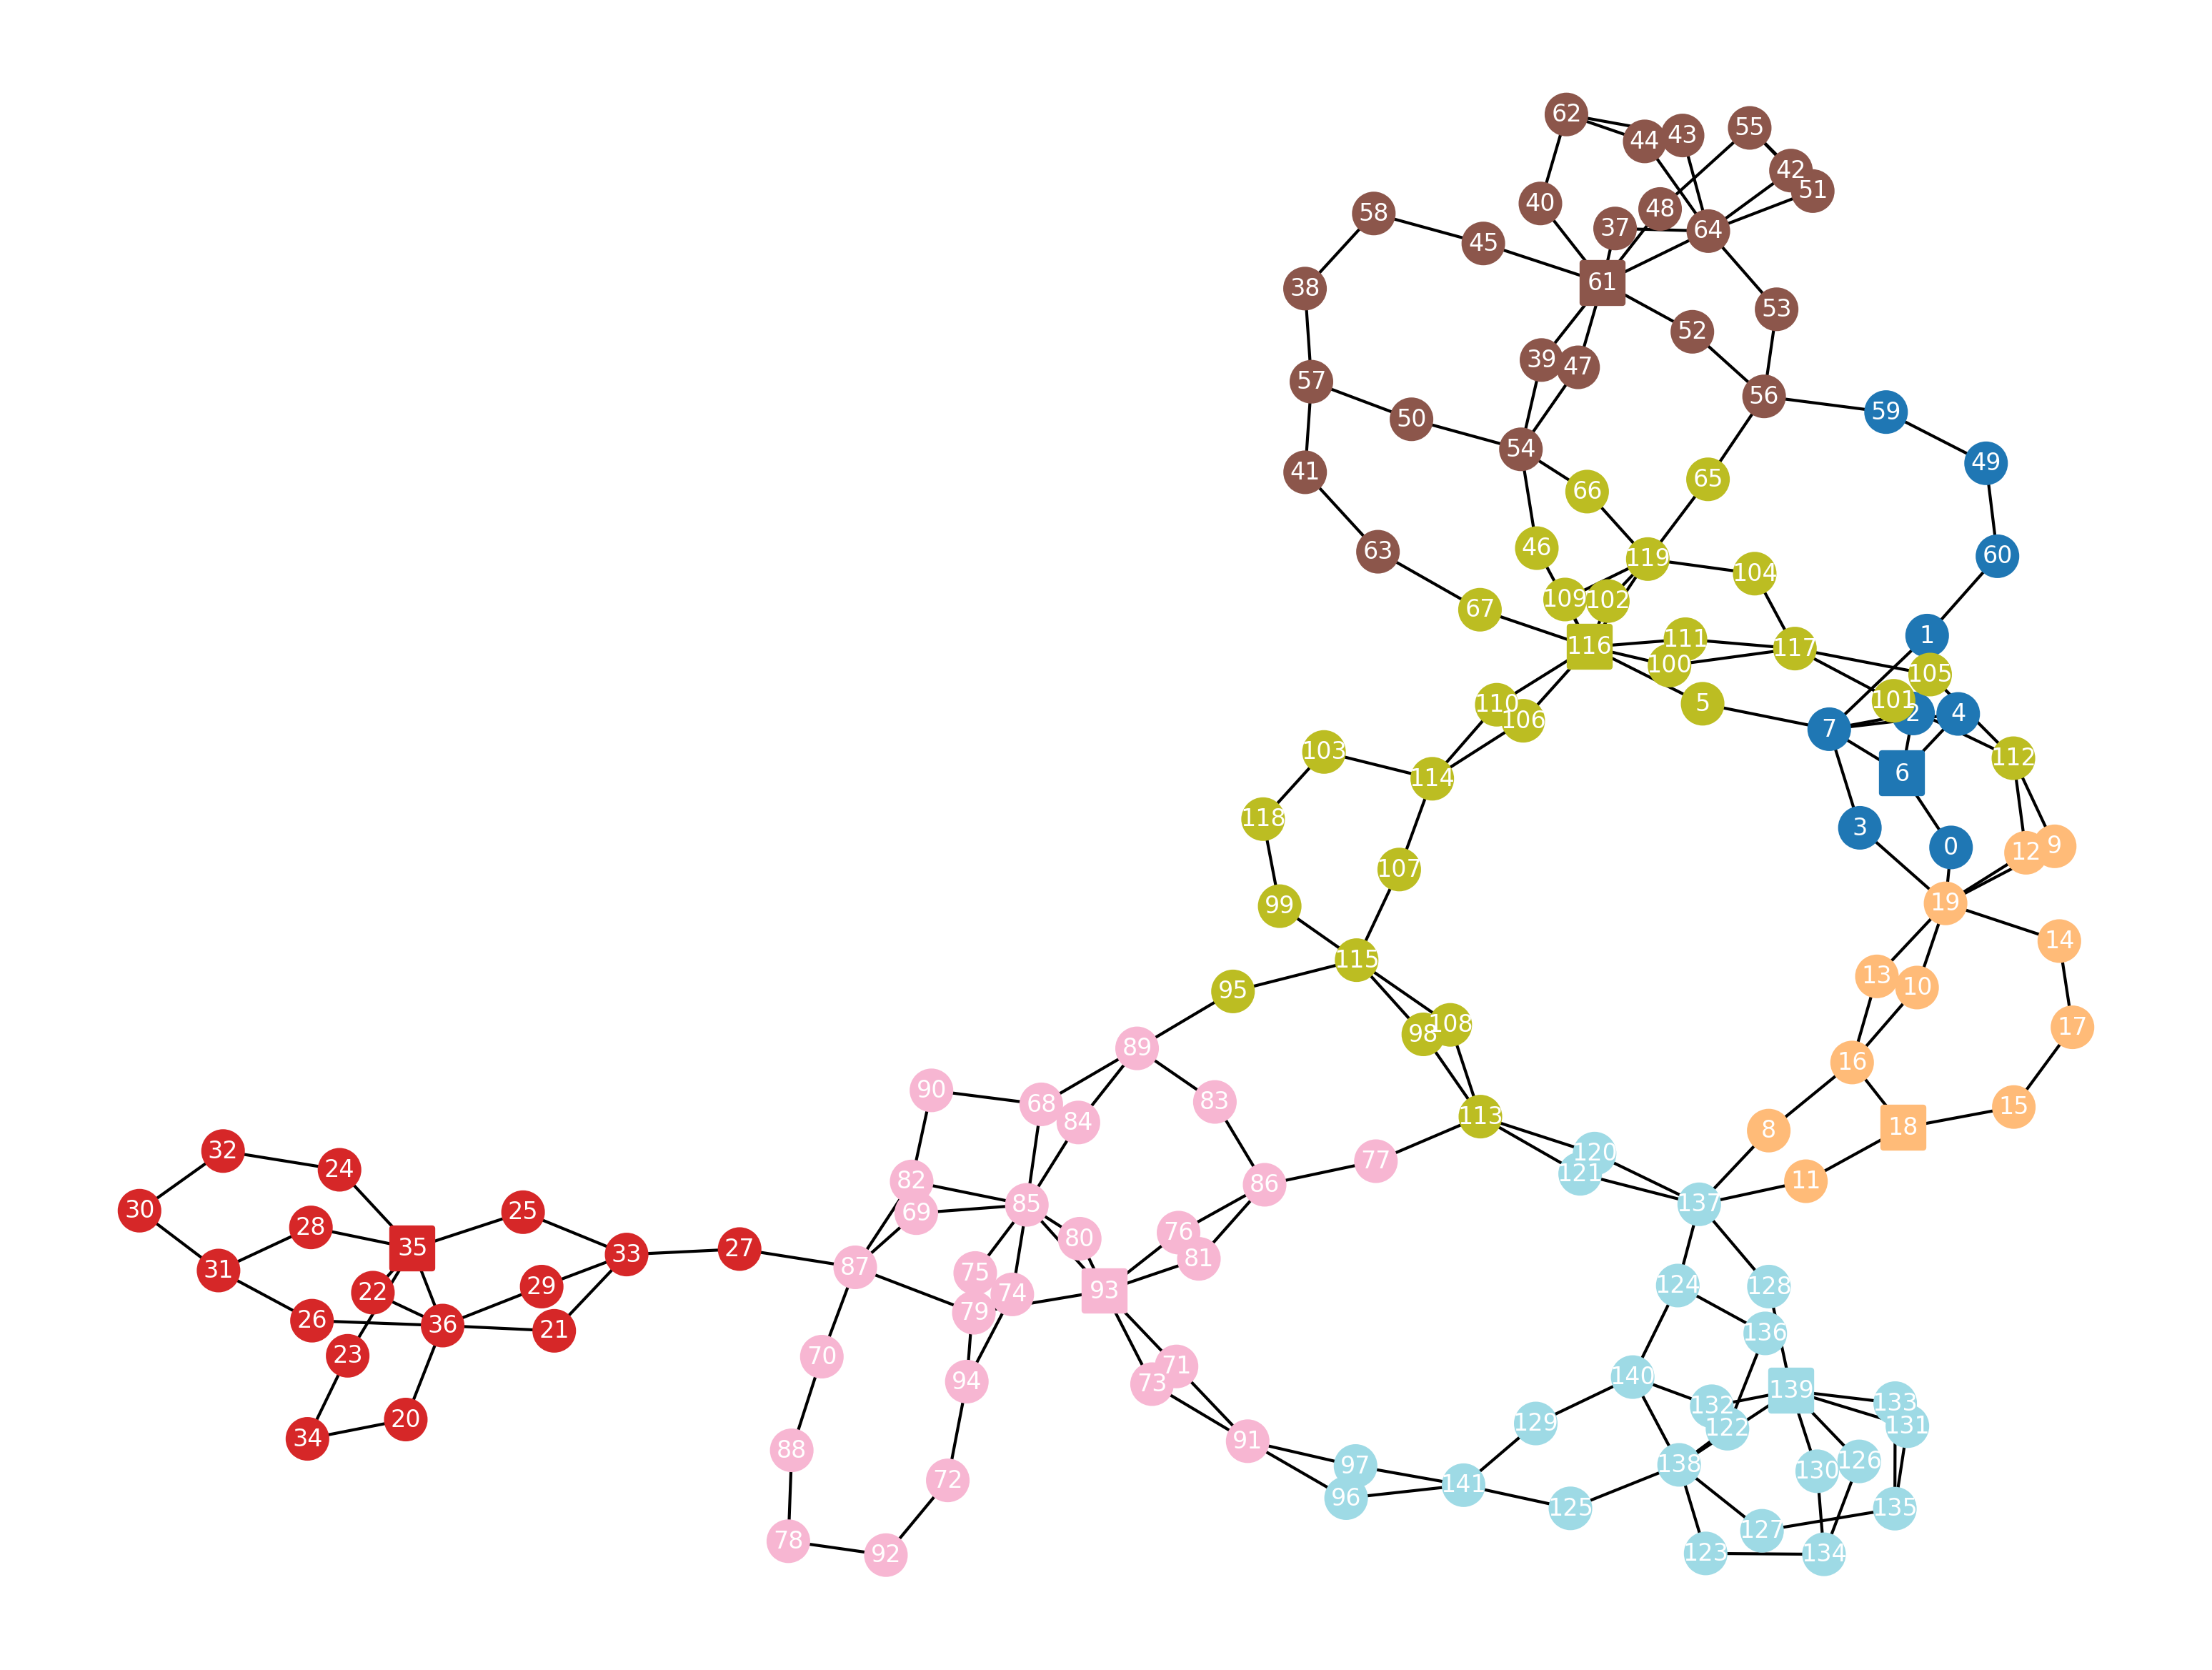
\includegraphics[width=.8\linewidth]{img/switchstate_exploring/urban2/topology_sss_patched.png}
    \end{center}
    \caption{
        Atomic islands of "Urban 2" grid area. Layout produced with
        Kamada-Kawai layout algorithm\autocite{kamada_kawai}.
    }
    \label{fig:appendix:urban2:topology_patched}
  \end{figure}

  \begin{figure}[H]
    \centering
    \begin{tabular}{lrr}
      \toprule
      & SSS & Best random switch state \\
      \midrule
      Score (x100) & 67.1 & 68.9 \\
      Min. Voltage (V) & 383.4 & 388.5 \\
      Max. cable utilization (\%) & 119.6 & 119.6 \\
      Avg. cable utilization (\%) & 21.0 & 20.5 \\
      Max. transformer utilization (\%) & 61.7 & 64.1 \\
      Avg. transformer utilization (\%) & 41.2 & 40.8 \\
      Toal line losses (kW) & 78.9 & 73.2 \\
      \bottomrule
    \end{tabular}
    \caption{
      Grid performance of SSS and best random switch case obtained
      through 1000 samples
    }
    \label{fig:result:urban2:table}
  \end{figure}
  
  \begin{figure}[H]
    \begin{subfigure}{.33\textwidth}
      \centering
      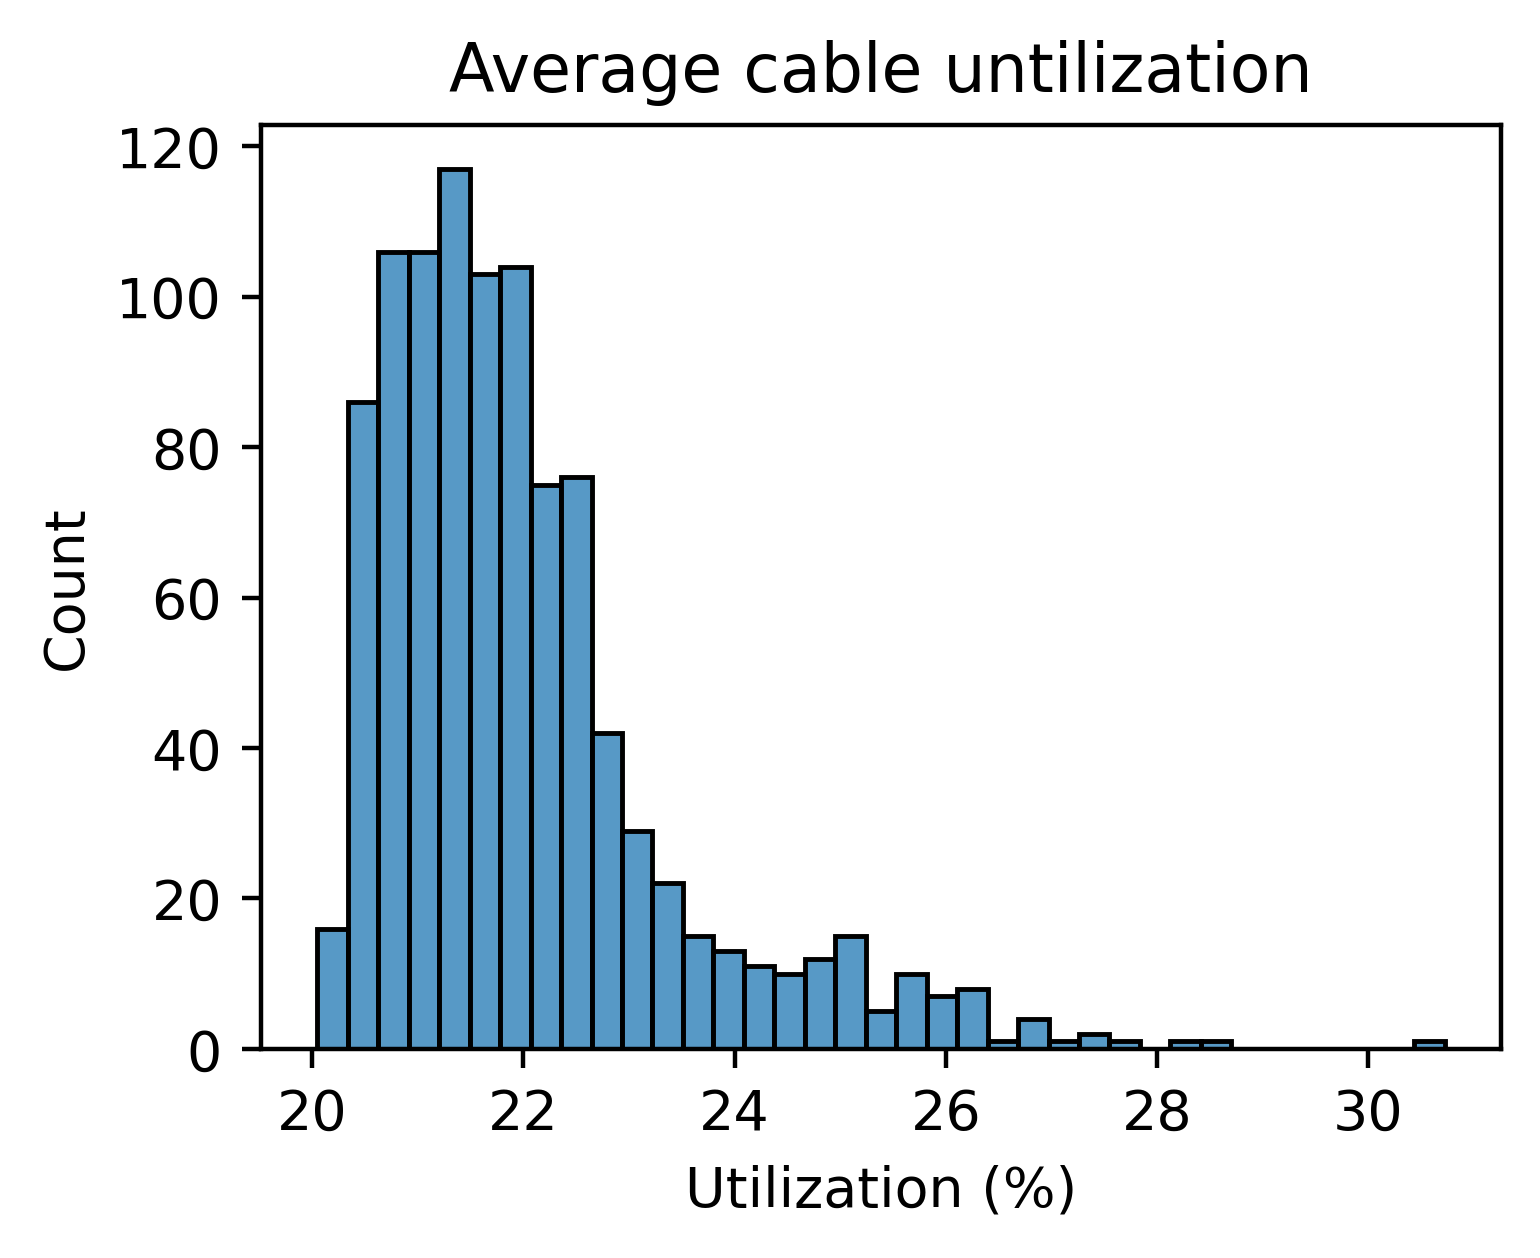
\includegraphics[width=\linewidth]{img/switchstate_exploring/urban2/histograms/avg_cable_util.png}
      \caption{}
      \label{fig:appendix:urban2:histograms:avg_cable}
    \end{subfigure}%
    \begin{subfigure}{.33\textwidth}
      \centering
      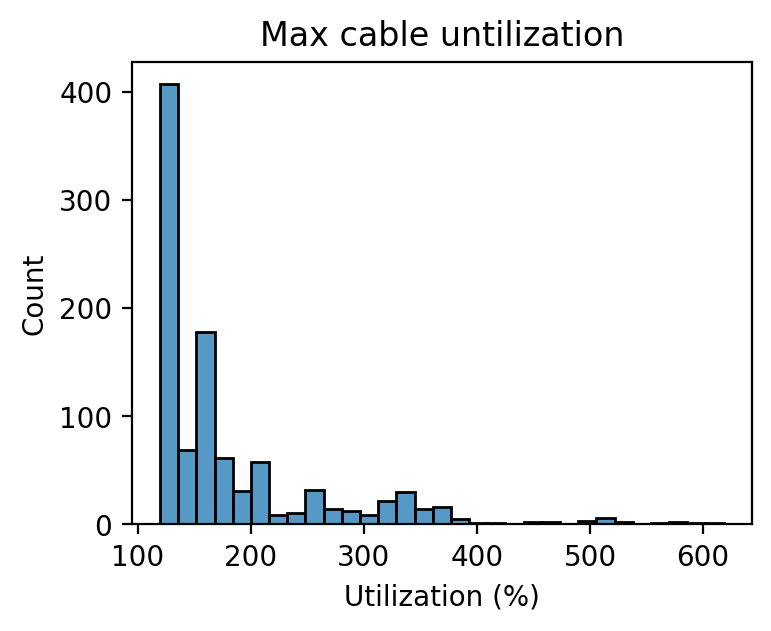
\includegraphics[width=\linewidth]{img/switchstate_exploring/urban2/histograms/max_cable_util.png}
      \caption{}
      \label{fig:appendix:urban2:histograms:max_cable}
    \end{subfigure}
    \begin{subfigure}{.33\textwidth}
        \centering
        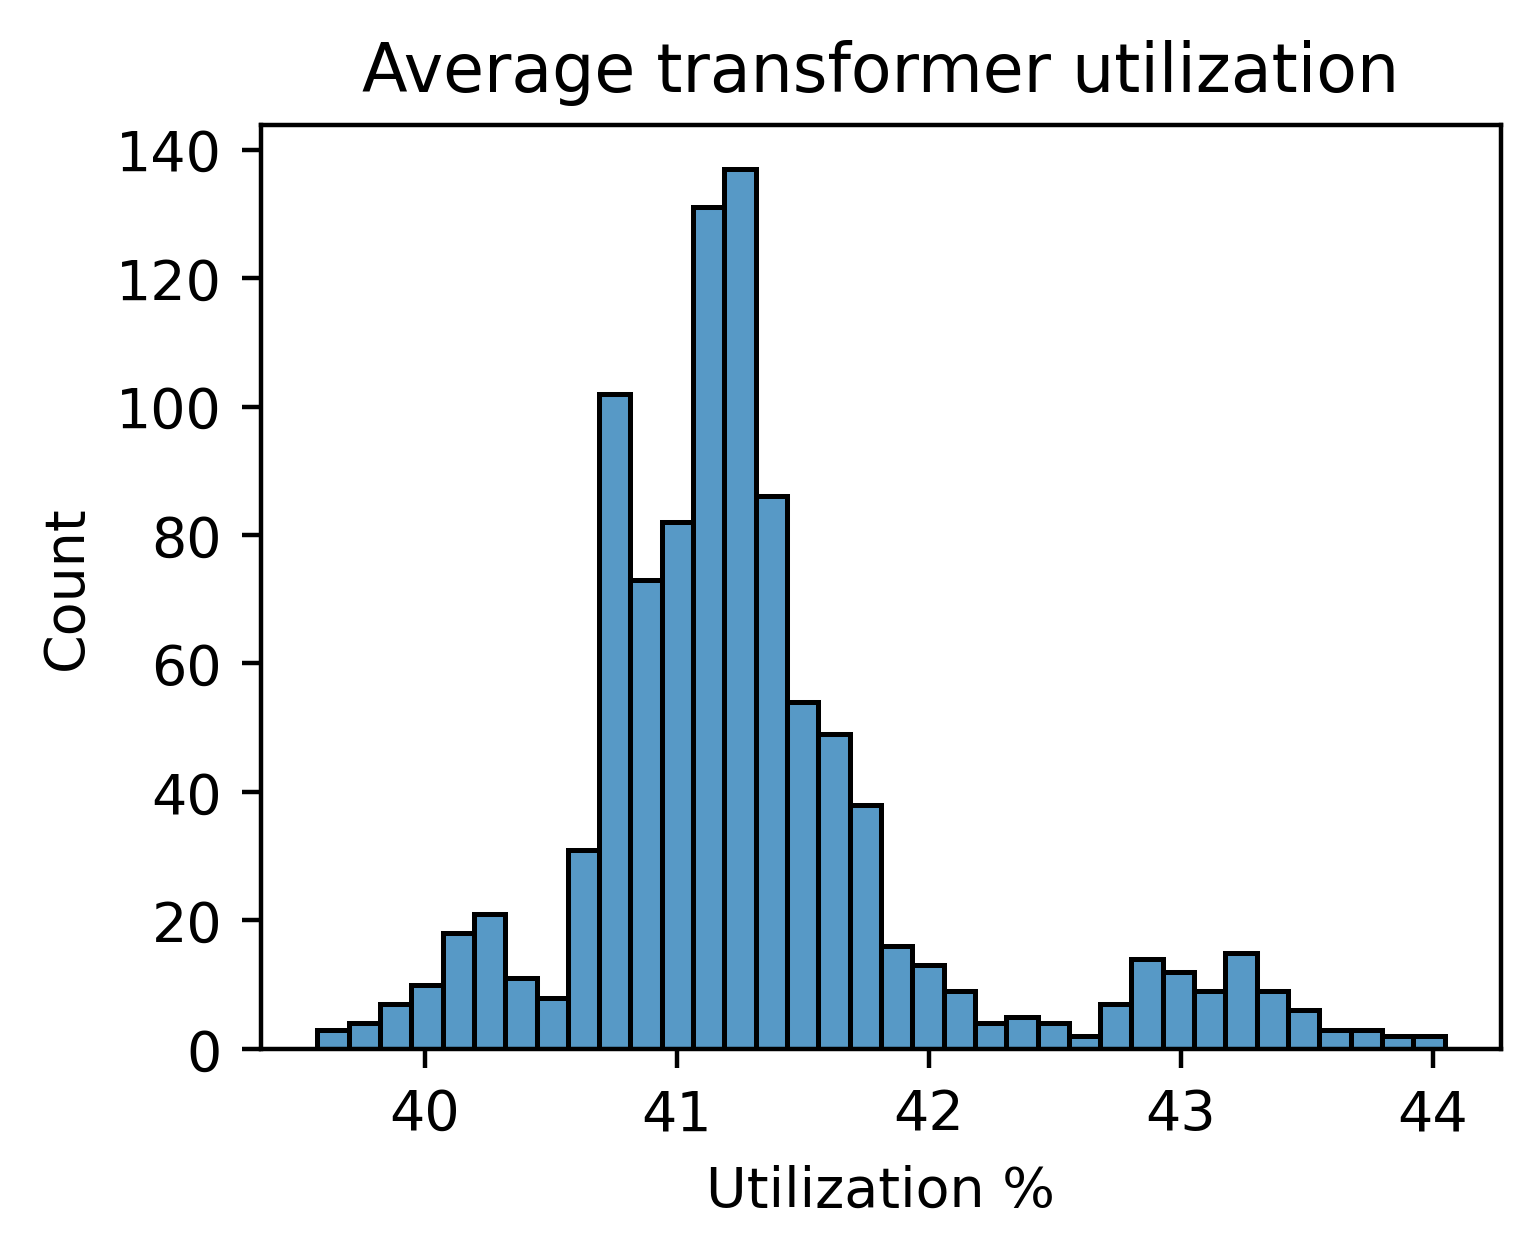
\includegraphics[width=\linewidth]{img/switchstate_exploring/urban2/histograms/avg_trafo_util.png}
        \caption{}
        \label{fig:appendix:urban2:histograms:avg_trafo}
      \end{subfigure}\\
      \begin{subfigure}{.33\textwidth}
        \centering
        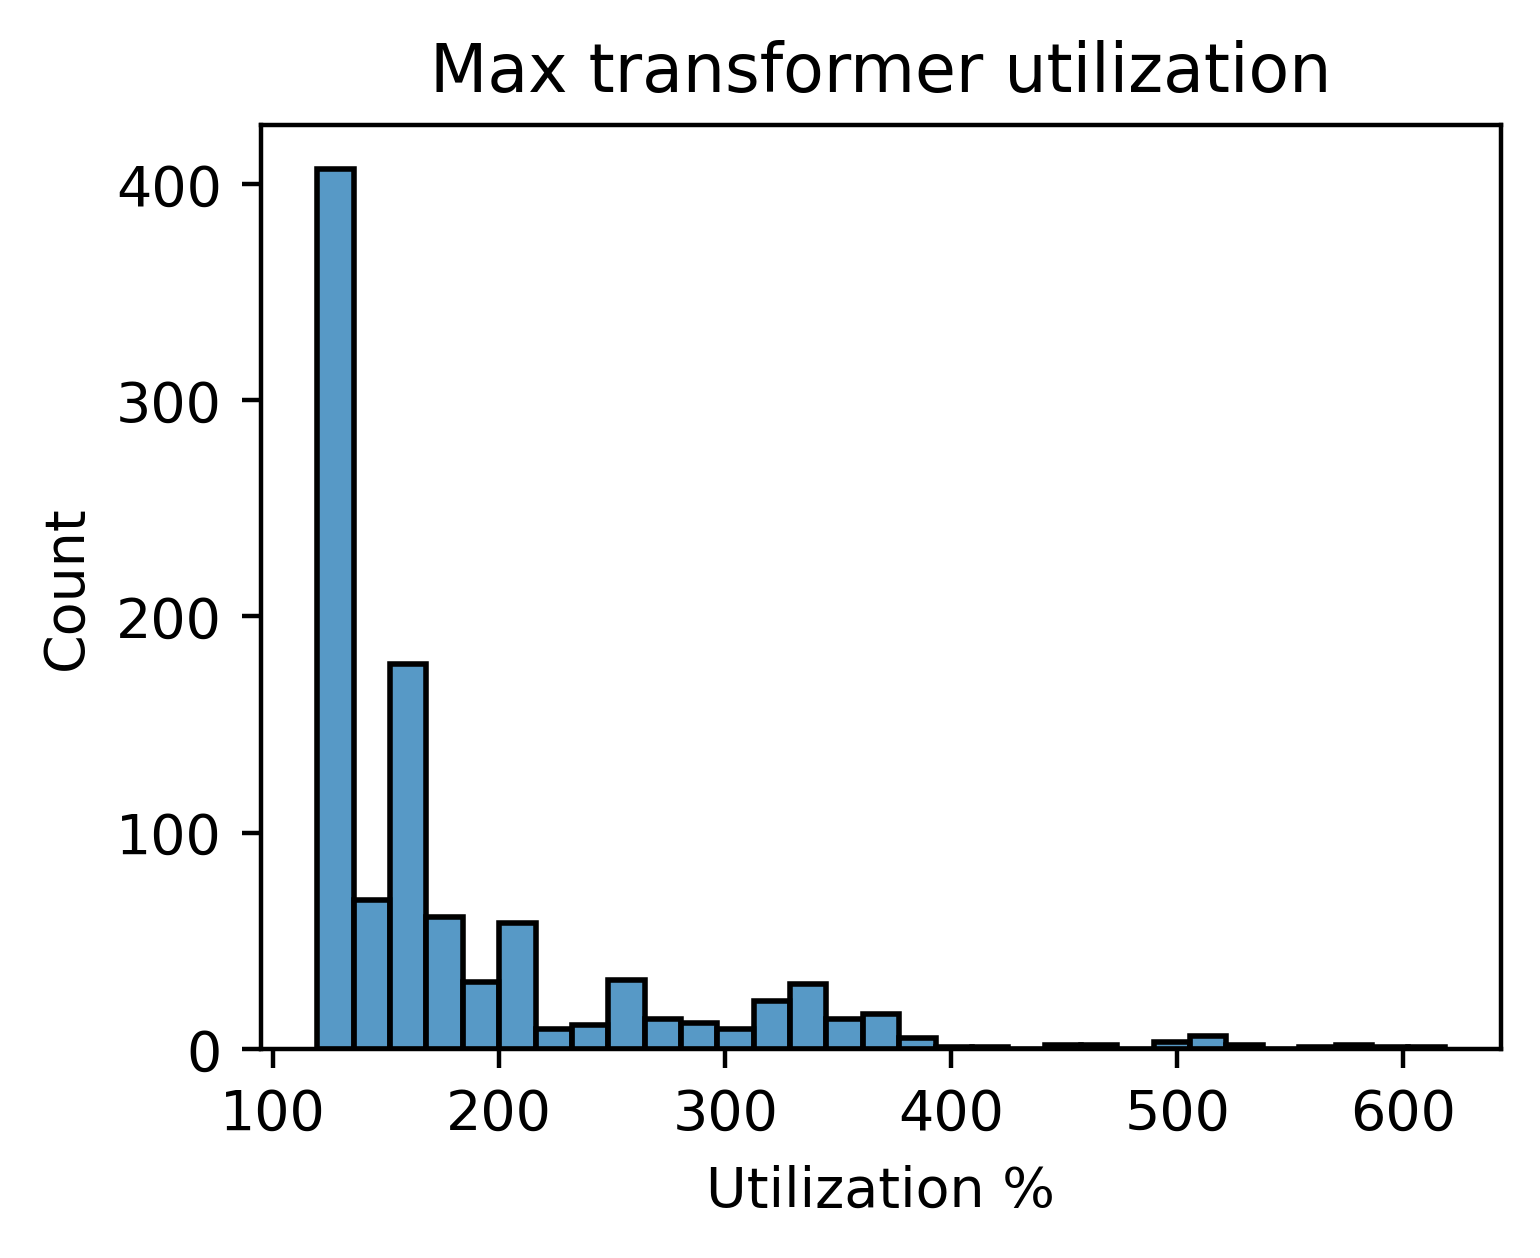
\includegraphics[width=\linewidth]{img/switchstate_exploring/urban2/histograms/max_trafo_util.png}
        \caption{}
        \label{fig:appendix:urban2:histograms:max_trafo}
      \end{subfigure}%
      \begin{subfigure}{.33\textwidth}
        \centering
        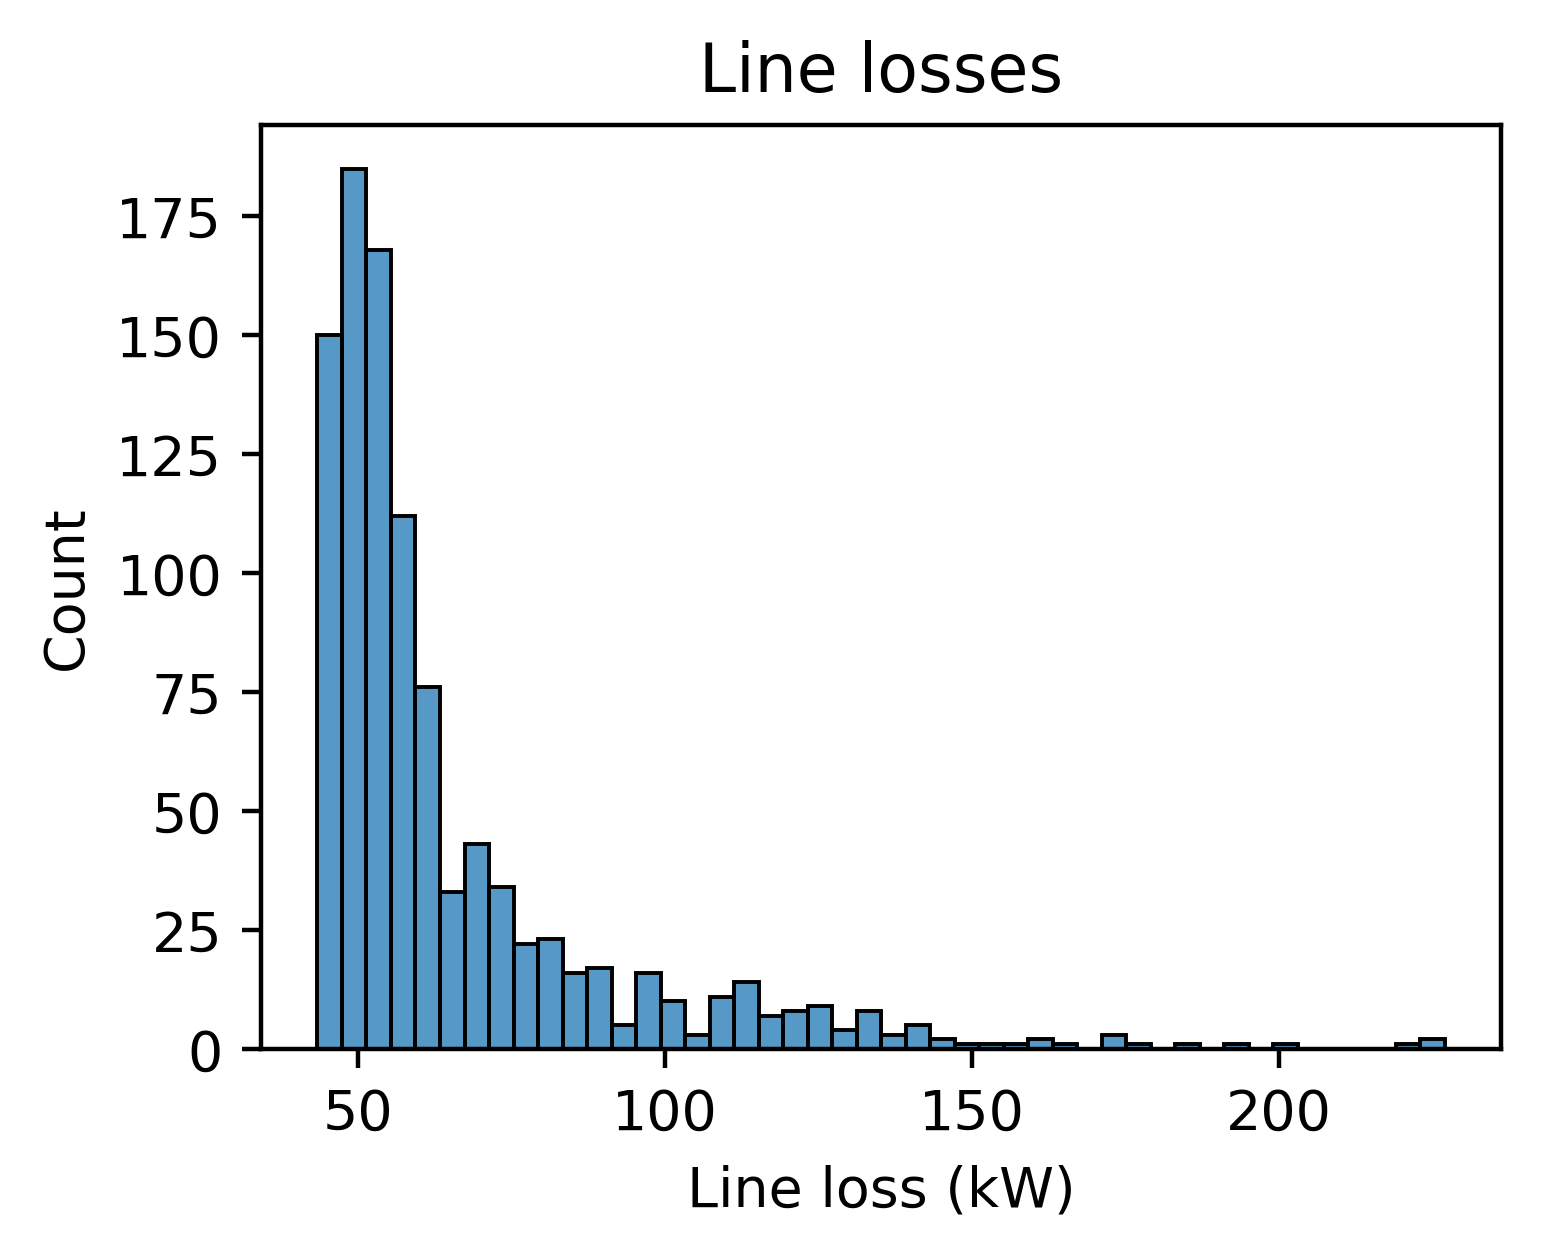
\includegraphics[width=\linewidth]{img/switchstate_exploring/urban2/histograms/line_loss.png}
        \caption{}
        \label{fig:appendix:urban2:histograms:line_loss}
      \end{subfigure}%
      \begin{subfigure}{.33\textwidth}
        \centering
        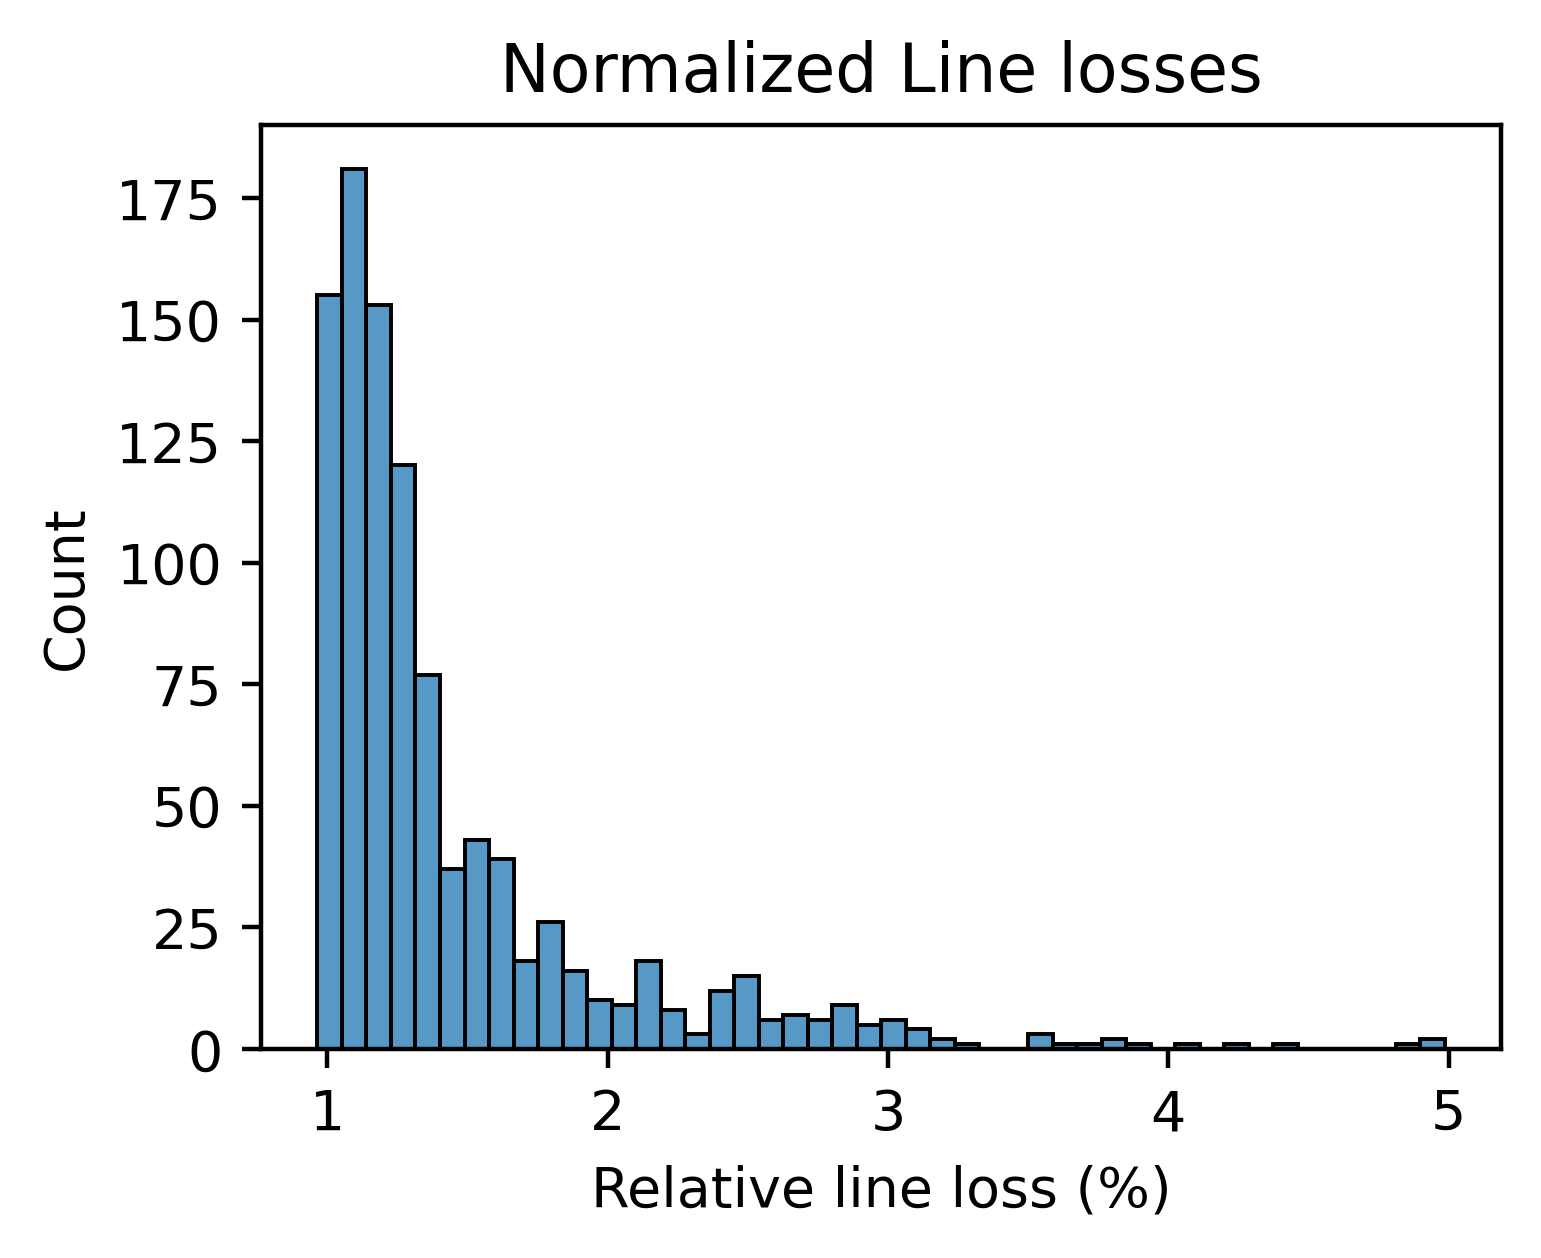
\includegraphics[width=\linewidth]{img/switchstate_exploring/urban2/histograms/line_loss_relative.png}
        \caption{}
        \label{fig:appendix:urban2:histograms:line_loss_rel}
      \end{subfigure}\\
      \begin{subfigure}{.33\textwidth}
        \centering
        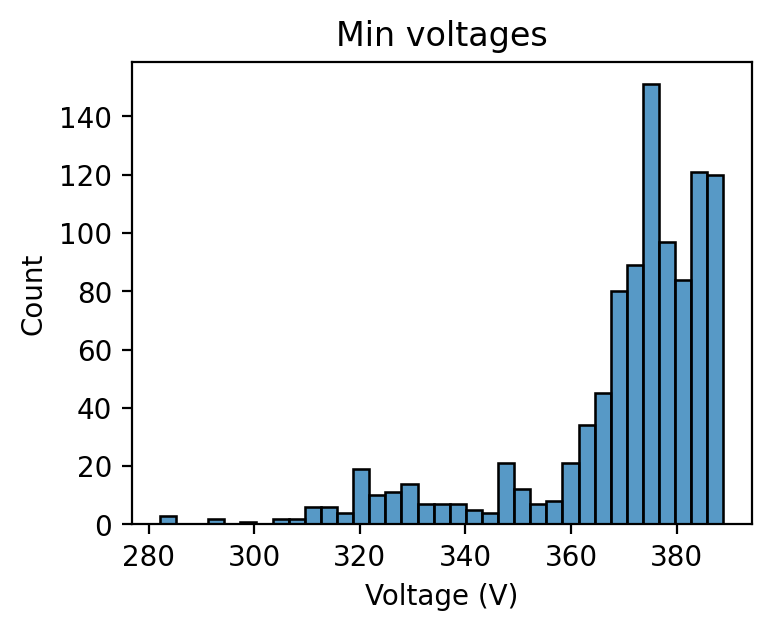
\includegraphics[width=\linewidth]{img/switchstate_exploring/urban2/histograms/min_voltage.png}
        \caption{}
        \label{fig:appendix:urban2:histograms:min_voltage}
      \end{subfigure}%
      \begin{subfigure}{.33\textwidth}
        \centering
        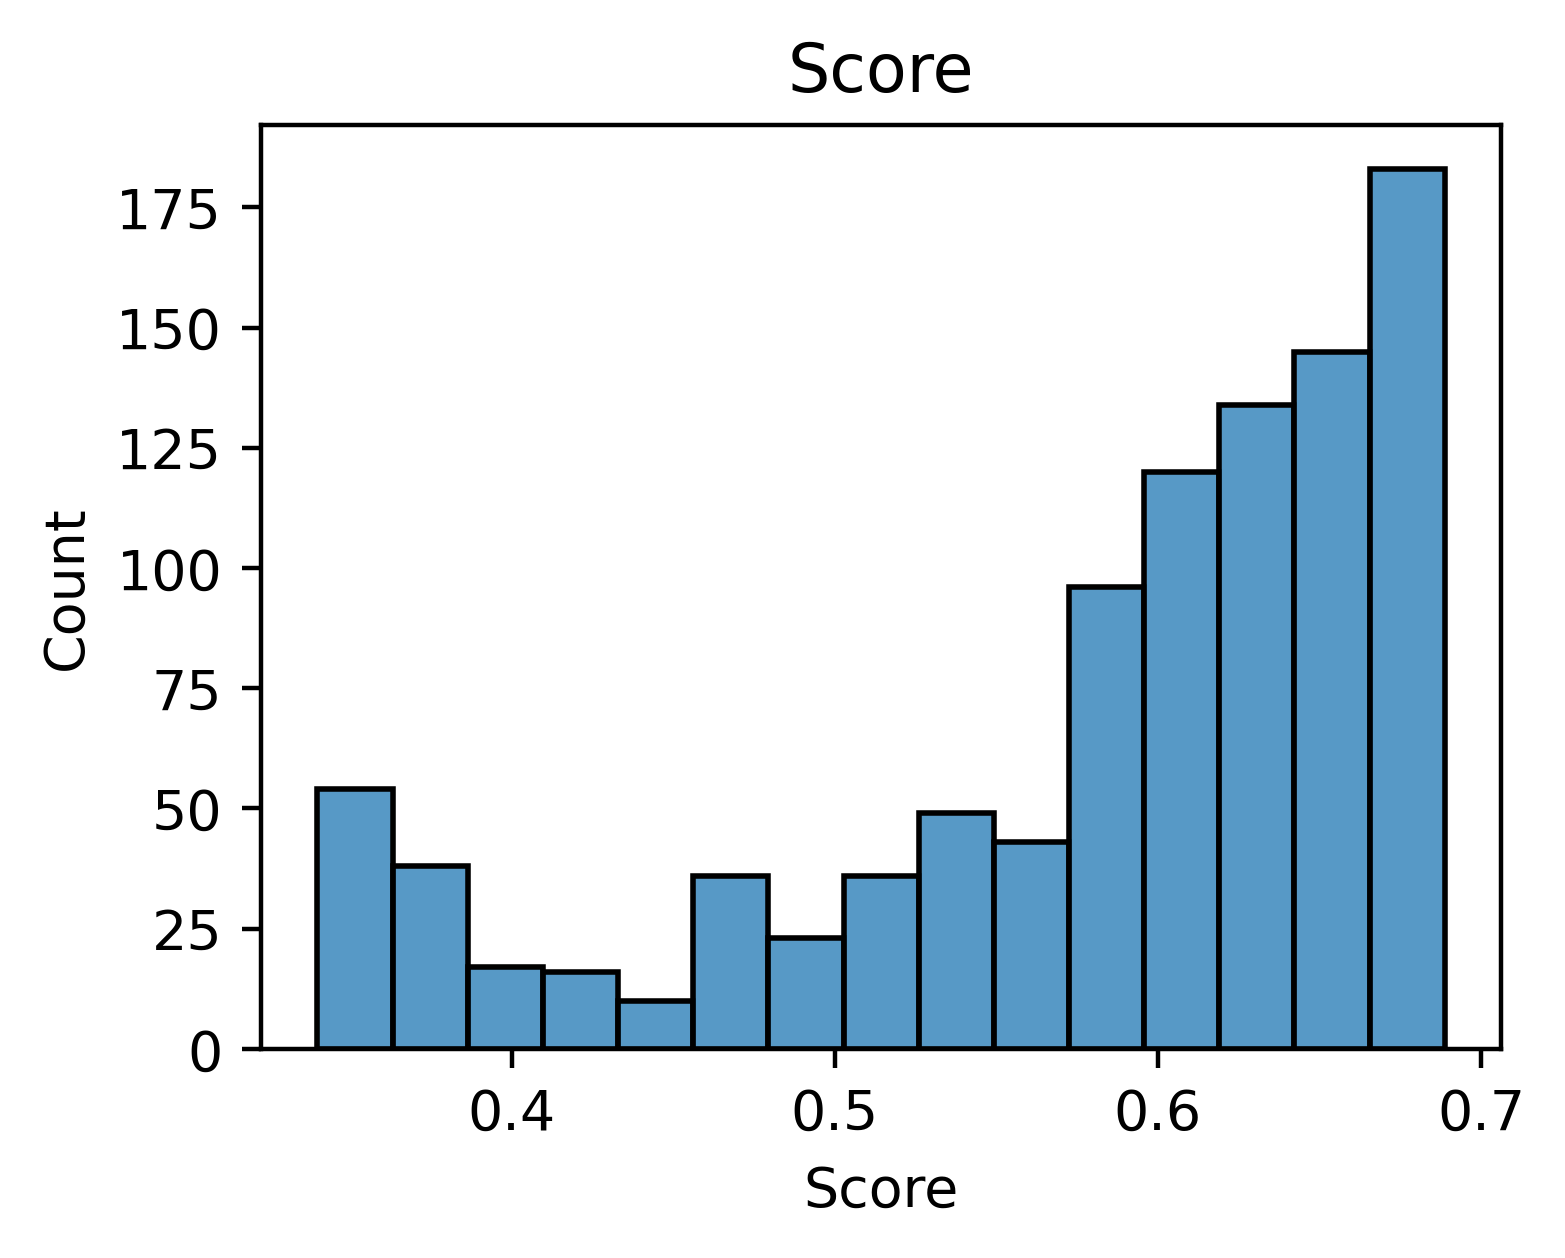
\includegraphics[width=\linewidth]{img/switchstate_exploring/urban2/histograms/score.png}
        \caption{}
        \label{fig:appendix:urban2:histograms:score}
      \end{subfigure}
      \caption{}
      \label{fig:appendix:urban2:histograms}
  \end{figure}

  \begin{figure}[H]
    \begin{subfigure}{.5\textwidth}
        \centering
        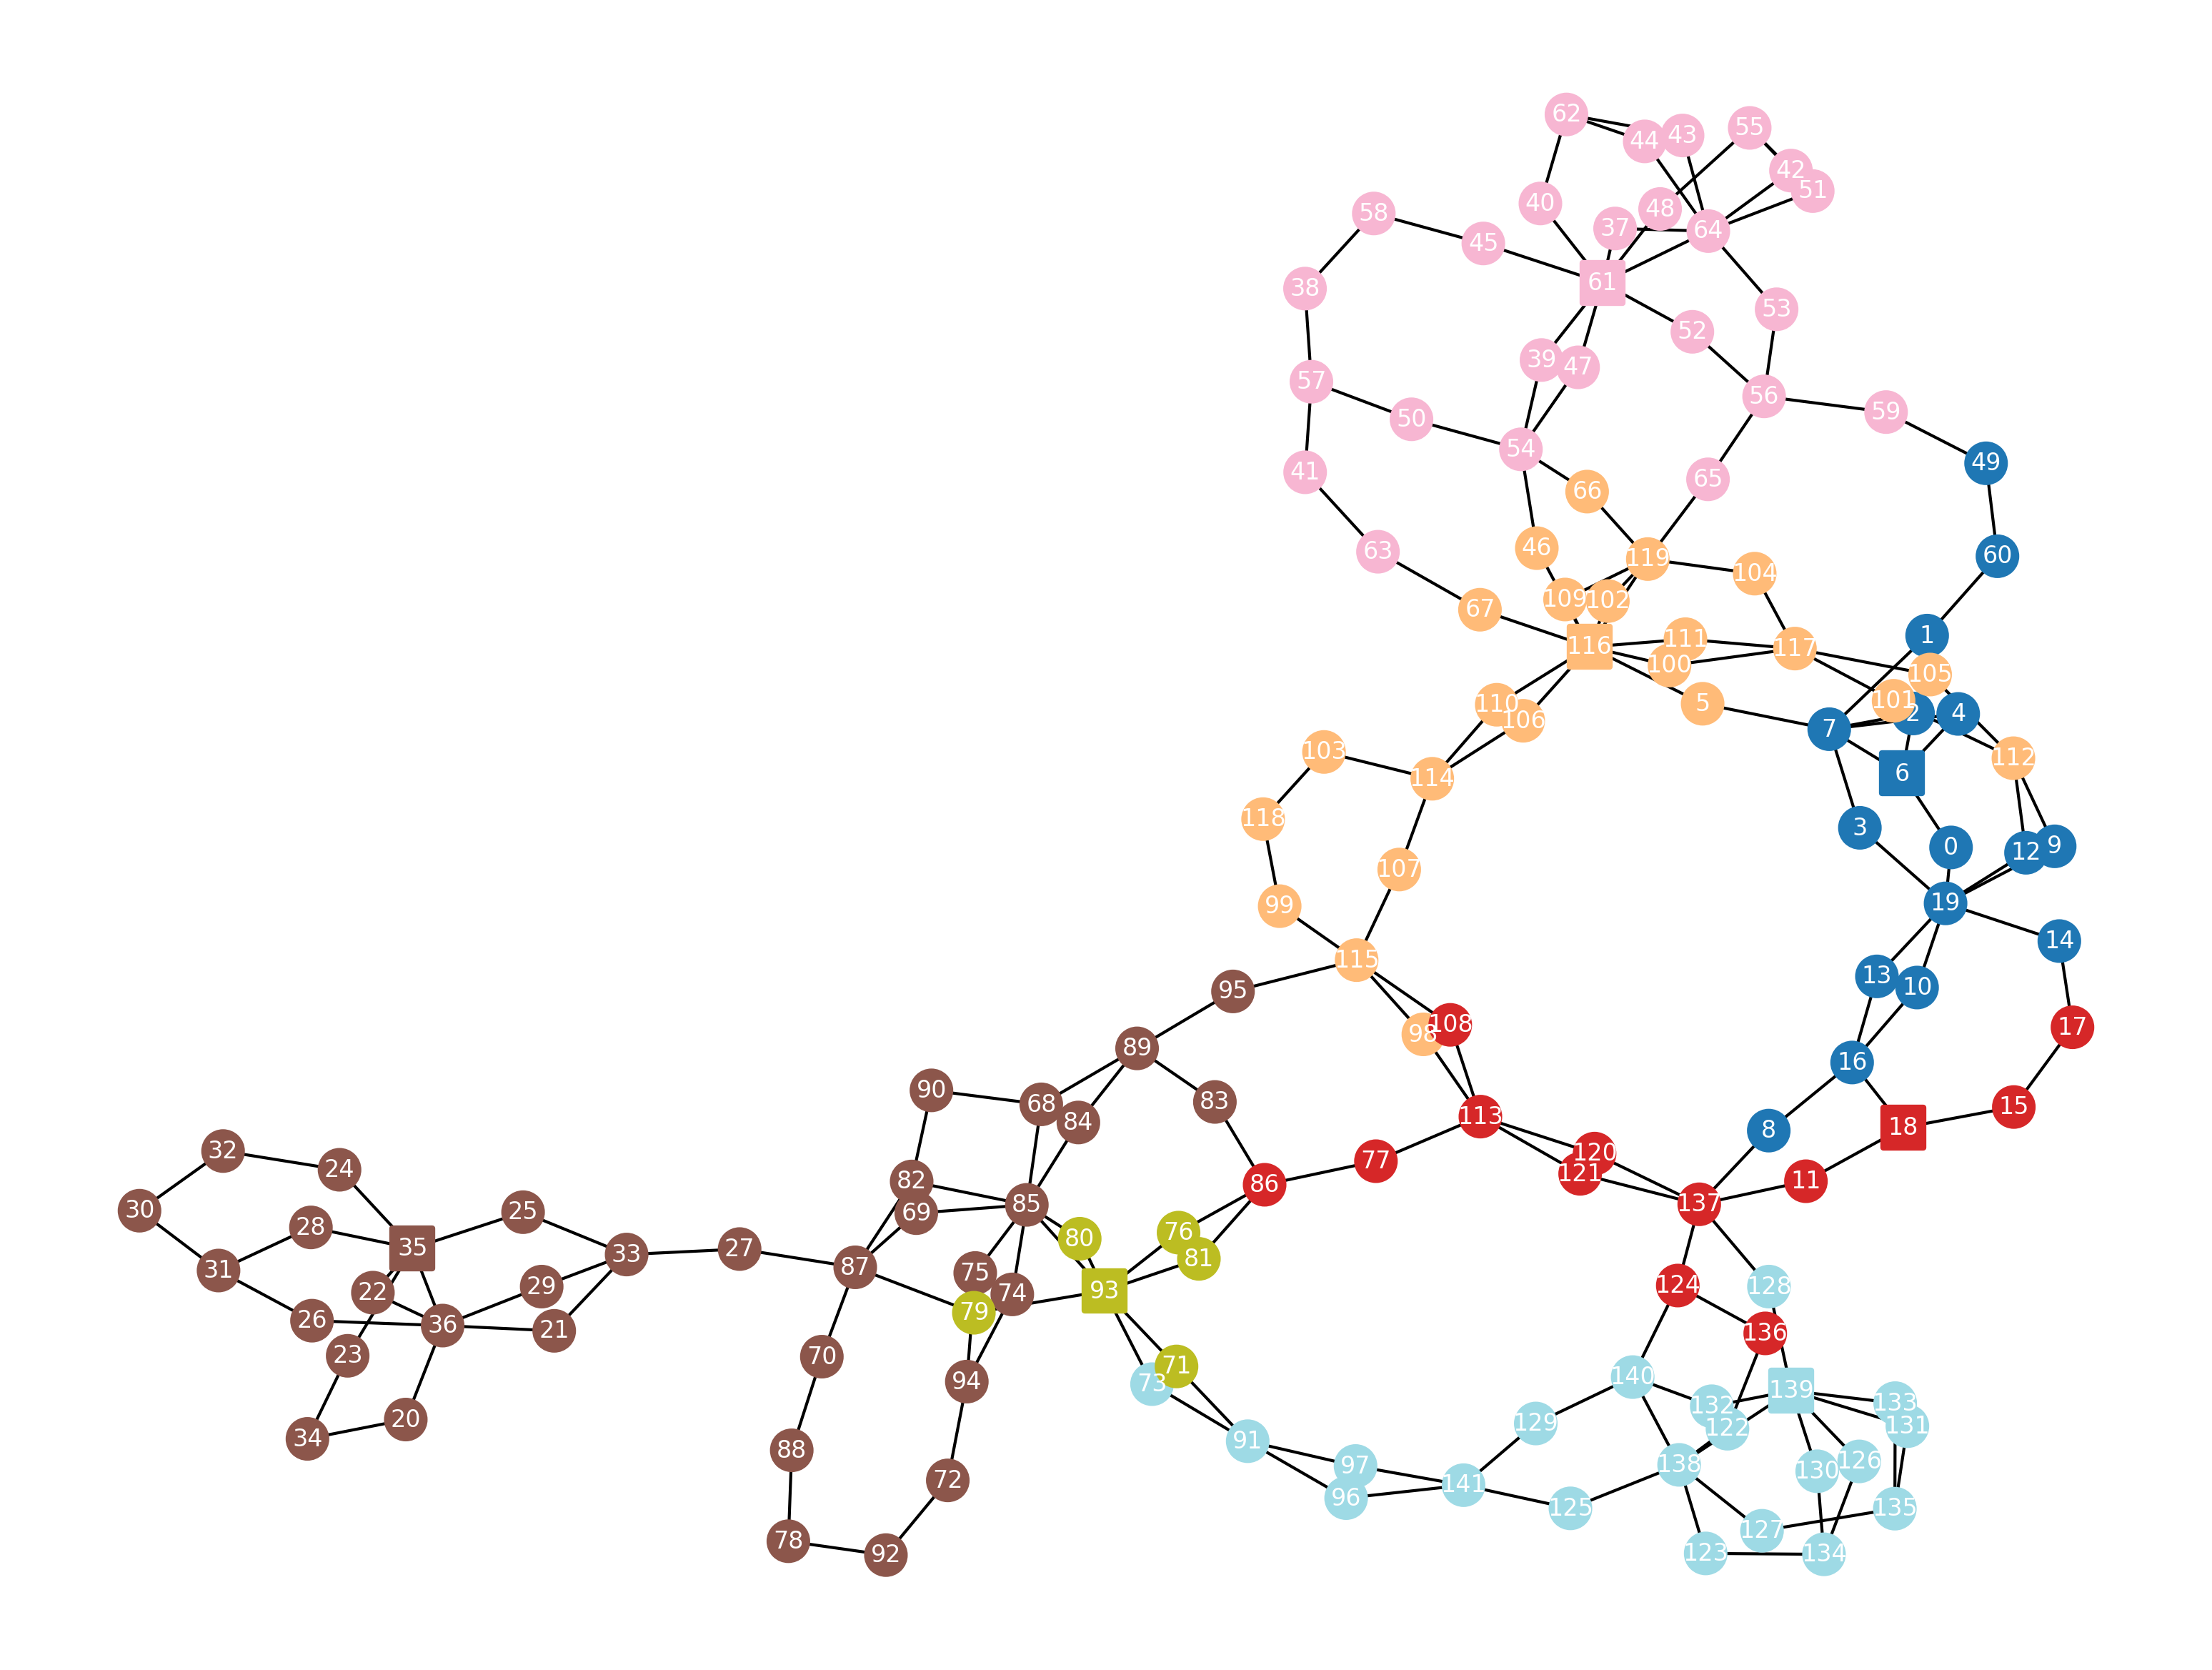
\includegraphics[width=\linewidth]{img/switchstate_exploring/urban2/topology_worst.png}
        \caption{}
        \label{fig:result:urban2:worst}
      \end{subfigure}%
      \begin{subfigure}{.5\textwidth}
        \centering
        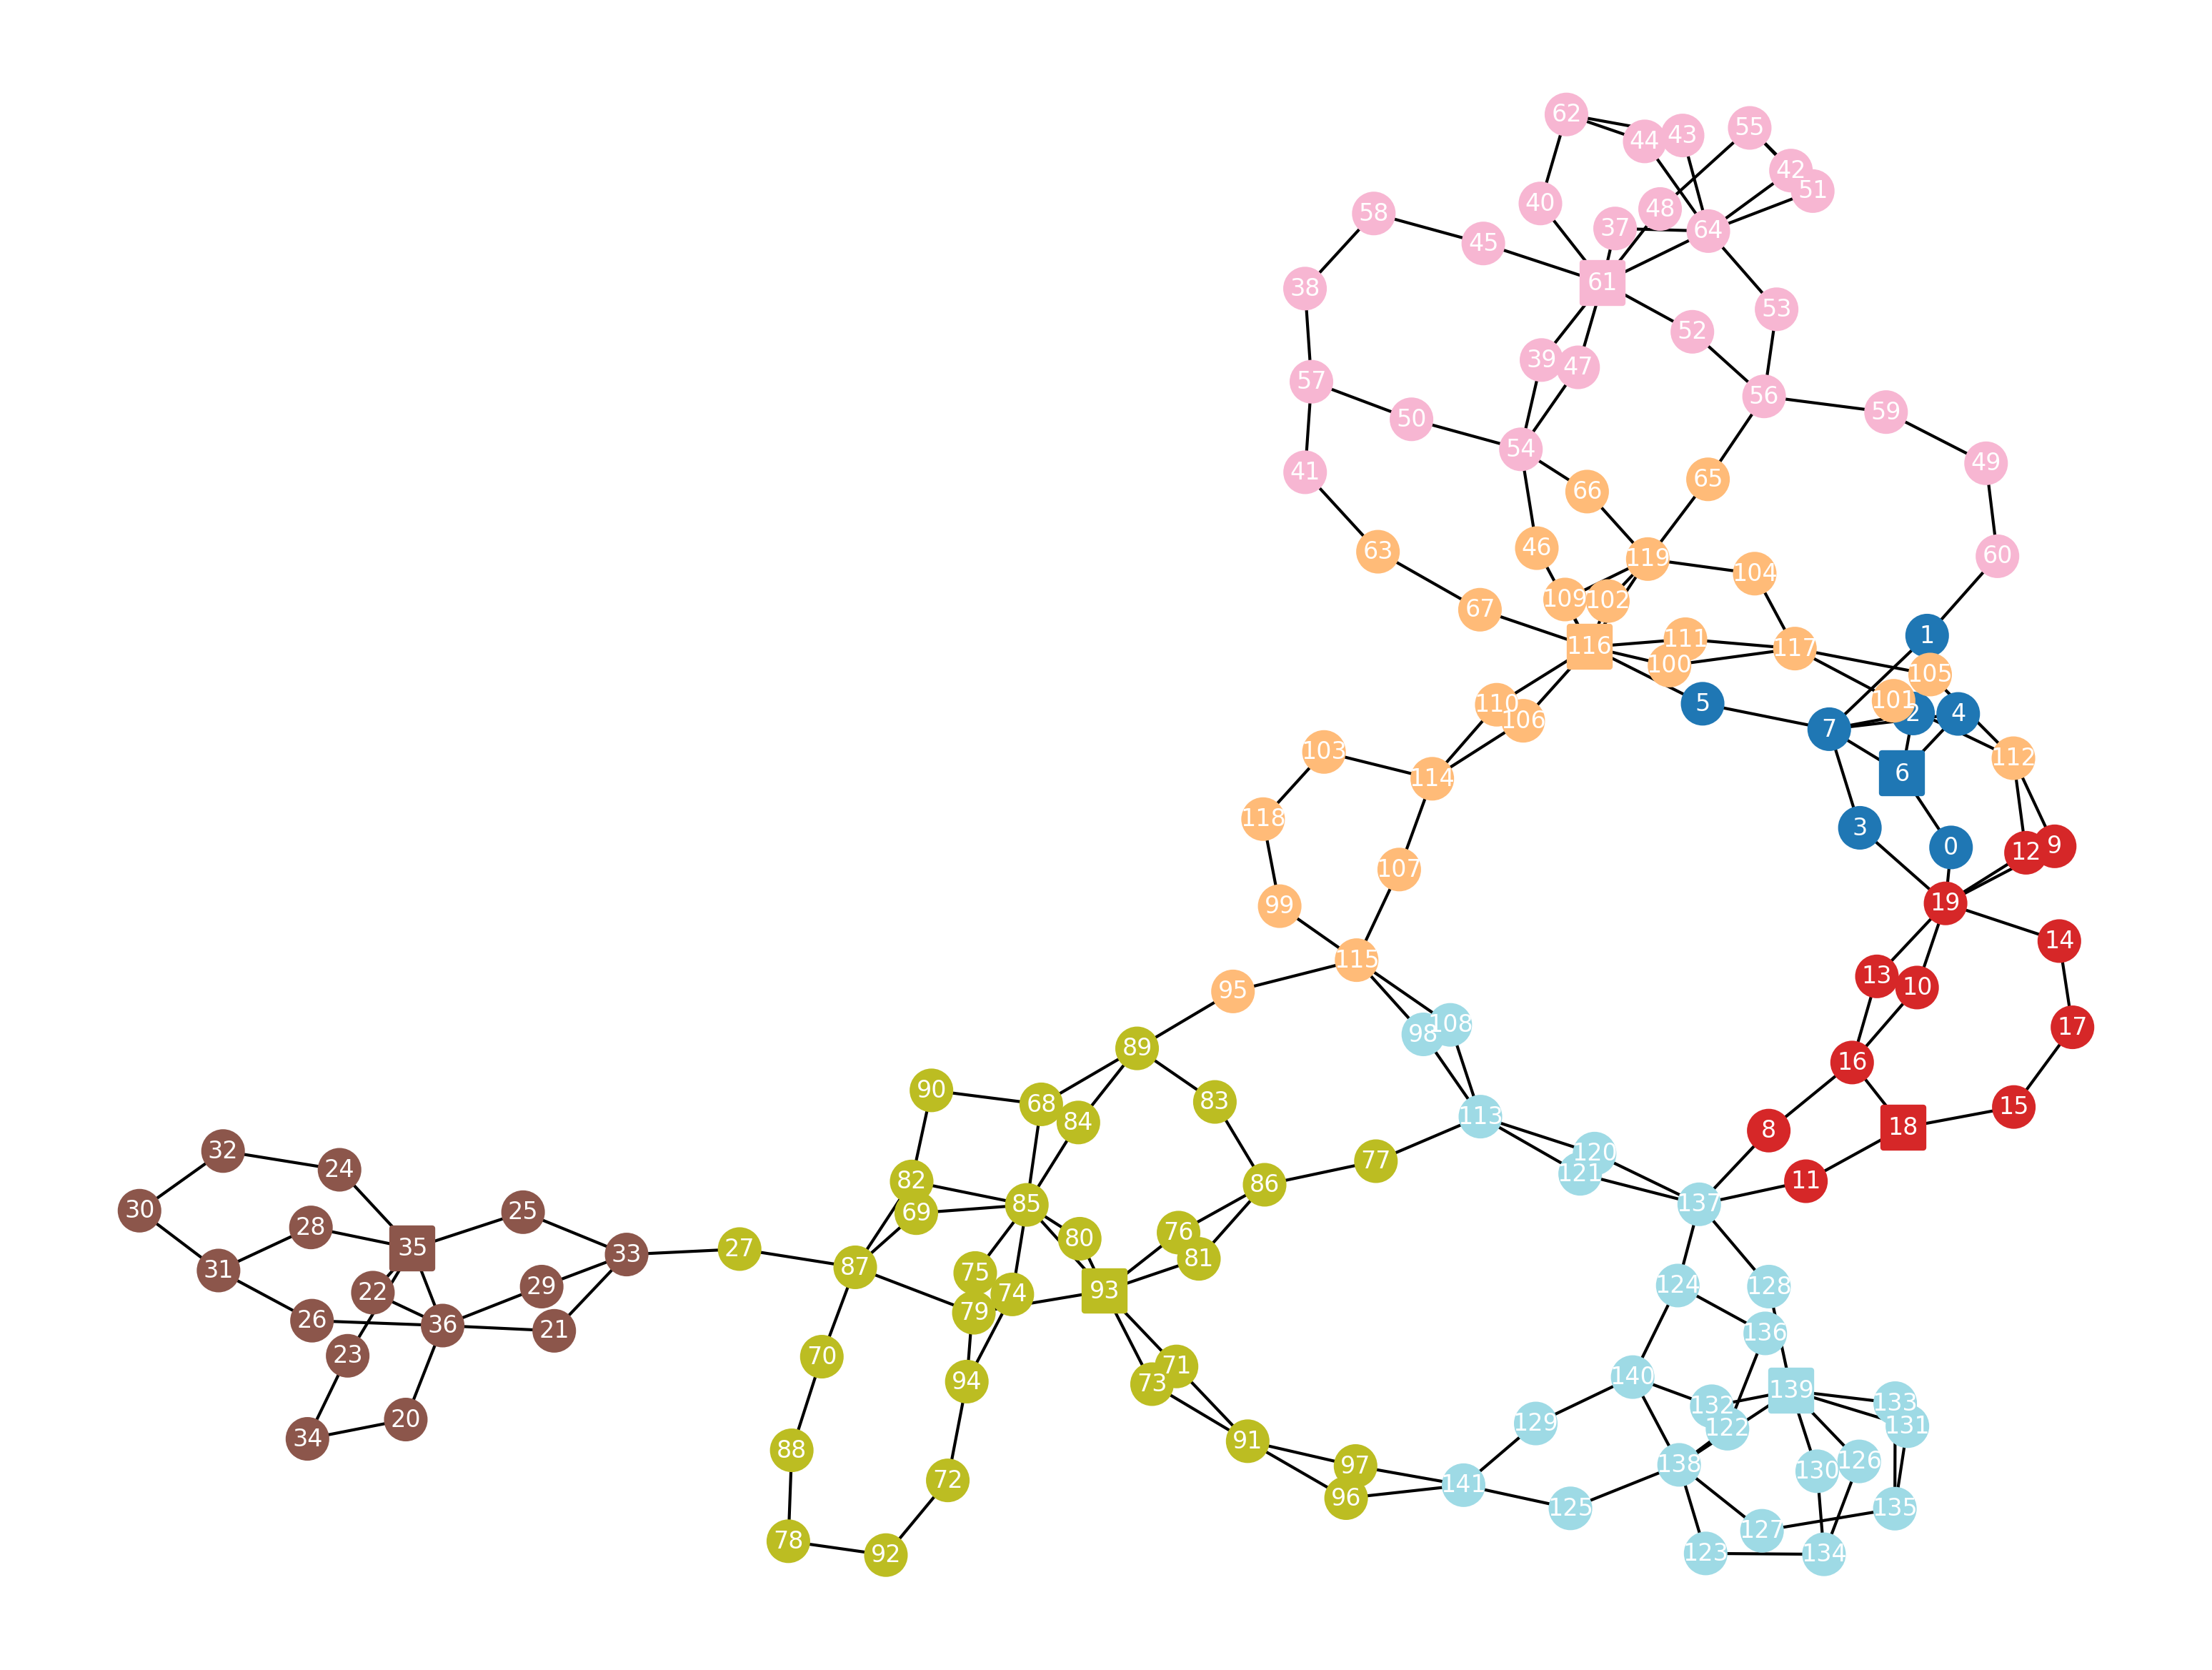
\includegraphics[width=\linewidth]{img/switchstate_exploring/urban2/topology_best.png}
        \caption{}
        \label{fig:result:urban2:best}
      \end{subfigure}
    \caption{
      Worst (a) and best (b) switch state found through random switch
      state generation in Urban 2 grid area. 
      Non-geographical layout using
      Kamada-Kawai algorithm\autocite{kamada_kawai}.
    }
  \end{figure}
  
  \begin{figure}[H]
    \begin{center}
        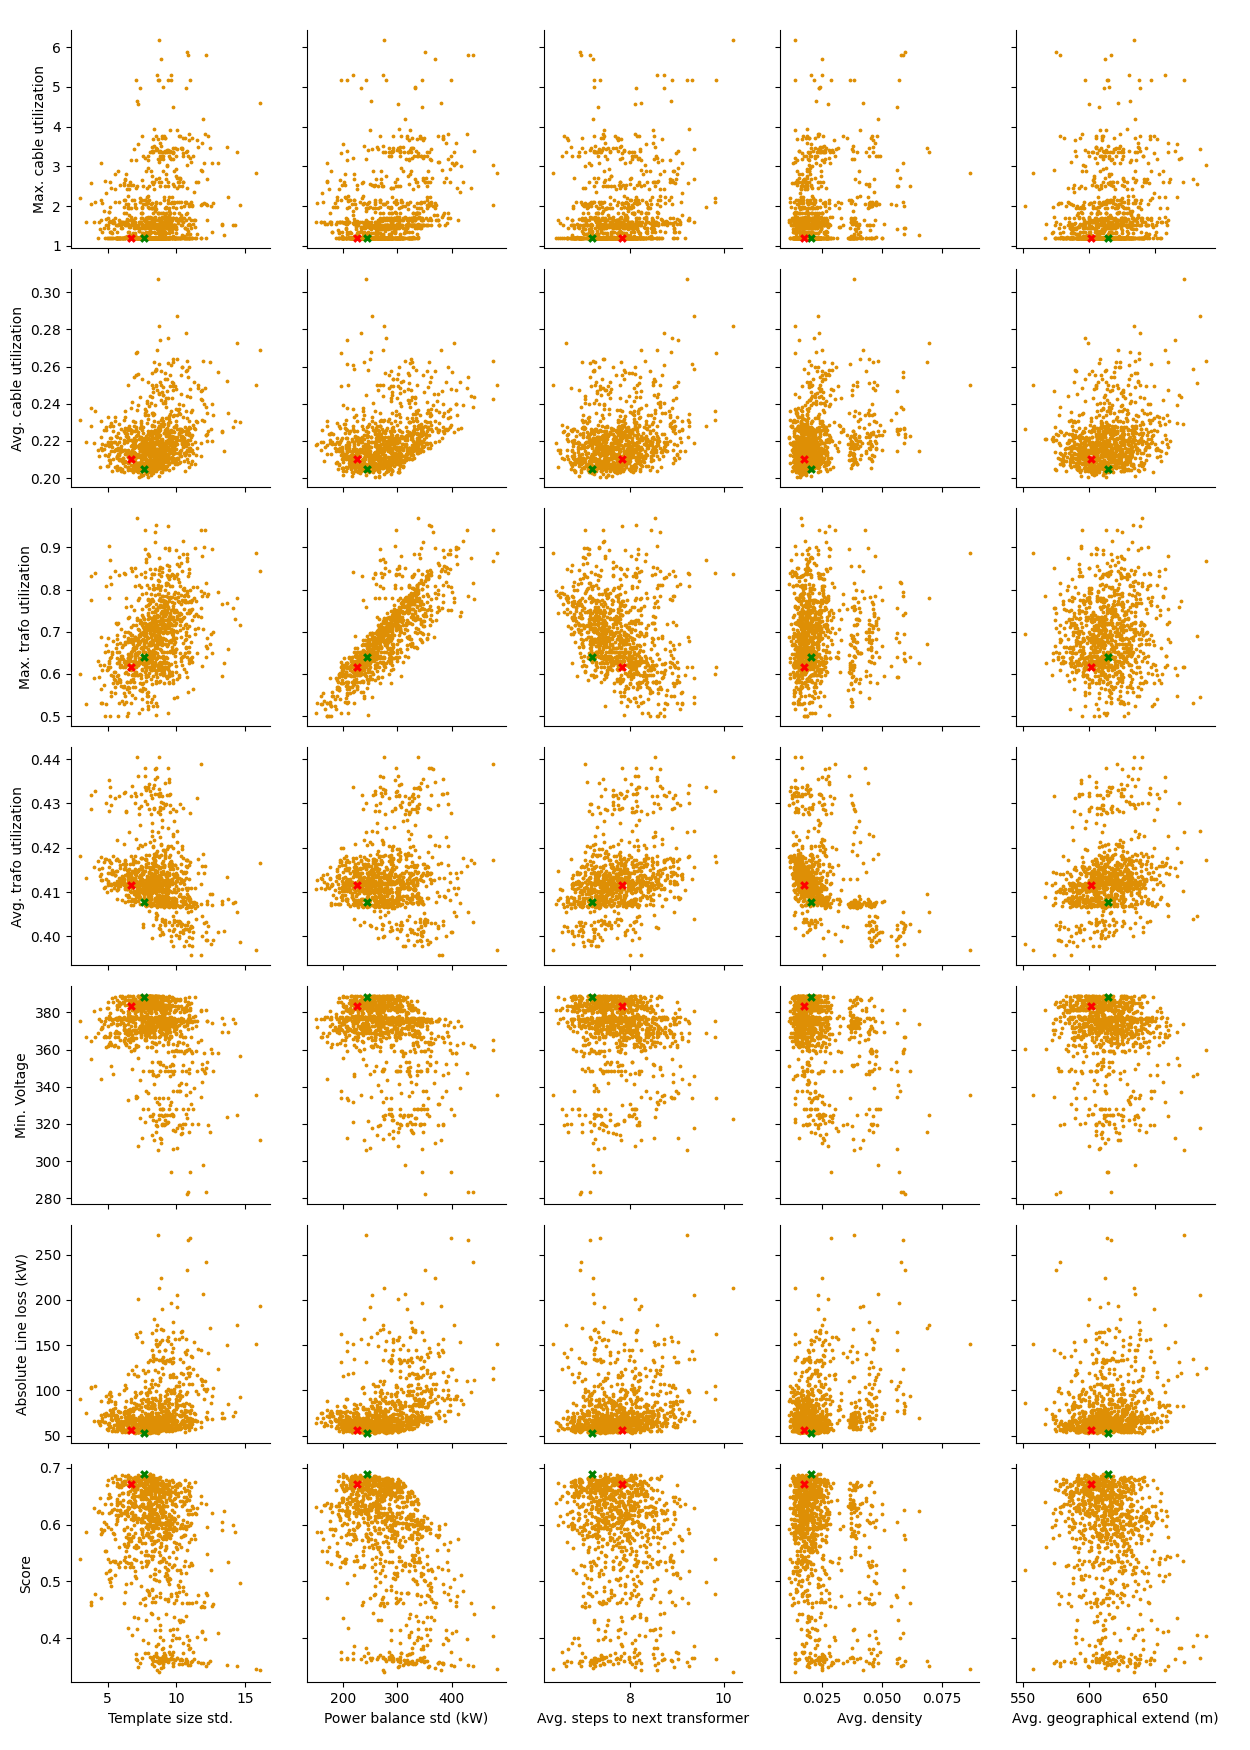
\includegraphics[width=\linewidth]{img/switchstate_exploring/urban2/correleation.png}
    \end{center}
    \caption{
      Correlation plots between topological/structural grid measures and 
      operational grid measures. Data points in red are the SSS and in green the best random switch state.
      Refer to \autoref{sec:measures} for more
      information on the individual measures.
    }
    \label{fig:appendix:urban2:correleation}
  \end{figure}